\begin{figure}[h]
    \centering
    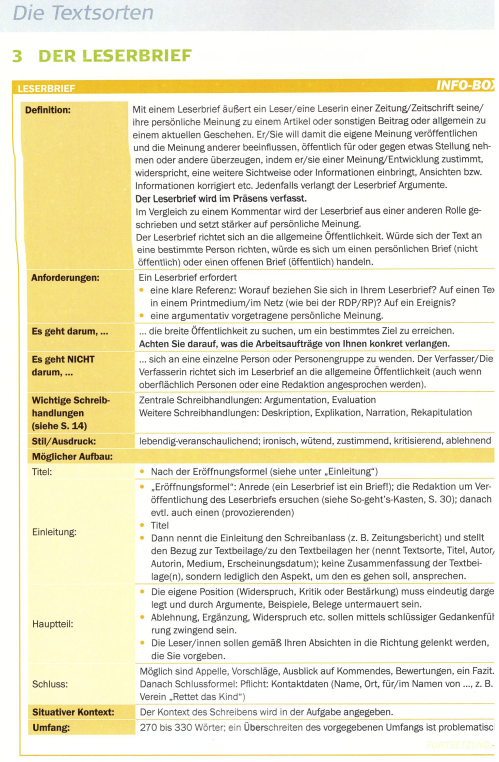
\includegraphics[scale=0.8]{./pics/Screenshot from 2023-02-06 12-28-25.png}
    \caption{Leserbrief: Definition + Aufbau}
    \label{fig:impl:Leserbrief1}
\end{figure}

\begin{figure}[h]
    \centering
    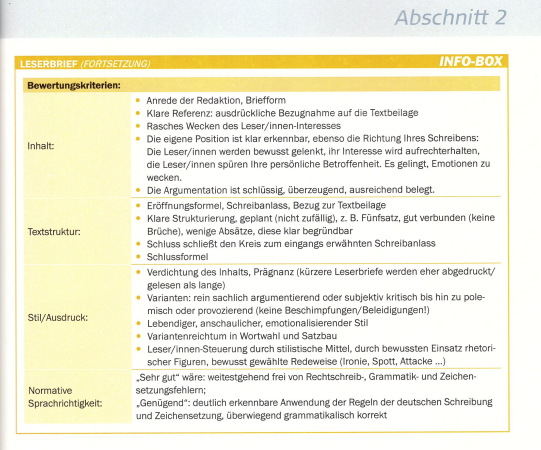
\includegraphics[scale=0.8]{./pics/Screenshot from 2023-02-06 12-28-55.png}
    \caption{Leserbrief: Verfassen}
    \label{fig:impl:Leserbrief2}
\end{figure}
\begin{figure}[h]
    \centering
    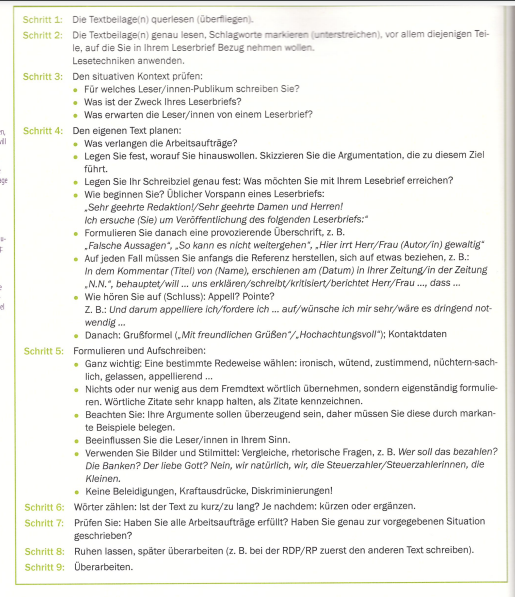
\includegraphics[scale=0.8]{./pics/Screenshot from 2023-02-06 12-29-05.png}
    \caption{Leserbrief: Fortsetzung}
    \label{fig:impl:Leserbrief3}
\end{figure}



\section{Mustertext}

Sehr geehrte Redaktion! 

Ich ersuche Sie um die Veröffentlichung des folgenden Leserbriefs: 
\subsubsection{Sexy und sexistisch  Muss das sein? }

Als ich die Kolumne „Sexy und sexistisch“ von Niki Glattauer, erschienen am 18. März 2013 in der Tageszeitung Kurier las, schoss mir sofort eine Frage durch den Kopf: Muss sowas denn wirklich sein?  

Herr Glattauer berichtet von einem sexistischen Werbeplakat der Wiener Linien. Darauf ist ein Mann zusehen, der seinen Allerwertesten direkt auf zwei elegant gekleidete Frauen, welche sich gerade unterhalten, gerichtet hat. Dabei sagt die eine Frau kichernd zu der anderen: Ich sagte doch, du sollst mehr Bus fahren. Niki Glattauer dreht daraufhin die Situation um und erläutert, dass ein Plakat mit zwei Männern in Anzug, die über den Hintern einer Frau feixen, ohne Berechtigung, als sexistisch oder unpassend abgestempelt werden würde. Herr Glattauers betont, dass ein klarer Unterschied zwischen sexy und sexistisch besteht. Denn das einzige, das vom Werbeplakat betont wird, ist der Hintern des Mannes. Kein Mann muss sich dadurch belästigt fühlen.  

Man kann das Ganze jedoch auch anders sehen. Die Ansicht, die man mit der Thematik verbindet, ist immer abhängig von den Gedanken oder Erinnerungen der Person. Manche Menschen ärgern sich über die Werbung und meinen sie sei unpassend und wieder andere lachen darüber und denken sich nichts weiter dabei.  

Da Sexismus leider auch heute noch immer eine sehr große Rolle in unserer Gemeinschaft spielt, muss man doch nicht mehr Wirbel über das Thema verbreiten, als ohnehin schon besteht. Ich gebe Herrn Glattauer mit der Überlegung, dass sexy nicht gleich sexistisch meint, zwar recht, jedoch kann man doch auf diese Anspielungen bei einer Werbung verzichten. Viele Leute fühlen sich dadurch persönlich angegriffen, beschämt oder gar verletzt und wohin sollen diese Gefühle bei der Debatte des Sexismus führen?  

\section{Eigener Text}
\subsection{Angabe}
\subsubsection{Körperbilder }

Verfassen Sie einen Kommentar. 

Situation: Im Rahmen eines Projekts Ihrer Klasse bzw. Ihres Kurses zum Thema Körperbilder verfassen Sie einen Kommentar, der auf der Projektwebsite veröffentlicht wird und für den Sie auch einen passenden Titel formulieren. 

Lesen Sie den Bericht Beauty-Apps: Die Macht der Influencer von Selina Thaler aus der OnlineAusgabe der Tageszeitung Der Standard vom 26. Jänner 2019 (Textbeilage 1). Verfassen Sie nun den Kommentar und bearbeiten Sie dabei die folgenden Arbeitsaufträge: 

\begin{compactitem}
    \item Geben Sie wieder, wodurch Selbstwahrnehmung und Körperbild laut Textbeilage beeinflusst werden.  
    \item Nehmen Sie dazu Stellung. 
    \item Bewerten Sie im Text genannte Maßnahmen und Initiativen, um der dargestellten Problematik entgegenzuwirken. 
\end{compactitem}

Schreiben Sie zwischen 270 und 330 Wörter. Markieren Sie Absätze mittels Leerzeilen.

\subsubsection{Beauty-Apps: Die Macht der Influencer }

Der Artikel von Selina Thaler über die Auswirkungen von Sozial Media und vor allem bearbeitet Bilder auf junge Frauen war einer der informativste Artikel, den ich seit Langem gelesen habe. Und dennoch frage mich, wieso ist das angesprochene Problem in der heutigen, aufgeklärten Zeit immer noch so ein Problem? 

Konkret geht es um die Auswirkungen, welche retuschierte Bilder auf unser Gehirn haben. Welche Folgen dies haben kann und dass es sogar Depressionen und starke Eifersucht auslösen kann. Und das ganz unterbewusst, ohne dass die Nutzer etwas davon mitbekommen. Vor allem die Vorbildfunktion der Influencer spielt hier eine starke Rolle. Viele jugendliche Mädchen, die selbst oft noch kein Selbstwertgefühl haben, wollen oft so perfekt aussehen wie die Menschen auf den Selfies auf Instagram. Snapchat-Dismorphia nennt man diese Unzufriedenheit, die durch die Verbreitung falscher und bearbeiteter Bilder ausgelöst wurden. 

Trotz geplanter Gegenmaßnahmen finde ich es schrecklich, dass durch Apps wie Instagram ein solch falsches Bild von dem menschlichen Körper an junge Menschen geliefert wird. Es ist schlimm, dass sich Mädchen abhungern oder Essstörungen aufbauen, nur um genauso dünn zu sein wie Models im Internet oder im Fernsehen. Doch viele dieser Fotos sind einfach bearbeitet und entsprechen nicht der Realität. Ich finde es gut, dass es schon Versuche gibt, solche Bilder zu markieren oder Models mit „Schönheitsfehler“ zu nehmen. Trotzdem müsste man meiner Meinung schon im Kindesalter die Menschen aufklären und über solche Fallen informieren. Denn trotz jeder Markierung, das Gehirn vergleicht sich trotzdem unterbewusst immer mit anderen. 

Ich rufe Sie, liebe Leser, dazu auf, ihre Söhne und Töchter darüber aufzuklären! Jeder sollte wissen, wie falsch Menschen auf Sozial Media sind, wie viele falsche Sachen viel zu viel Aufmerksamkeit bekommen, und vor allem, dass jeder Körper schön ist. Egal wie er geformt ist, wie viel man wiegt und wie groß die Kurven von jemanden sind. 

302 Wörter 

\newpage


\section{Formulierungshilfen}

Aufbau eines Leserbriefs: 
\begin{compactitem}
    
    \item Anrede: z.B. Name des Redakteurs: Sehr geehrter Herr Schuster! 
    \item Genaue Angabe des Artikels, auf den du dich beziehst: Datum und Überschrift des Artikels, Erscheinungsort 
    \item Schreibabsicht 
\end{compactitem}
So könntest du beginnen: 
\begin{compactitem}
    \item Sie schreiben in Ihrem Artikel (Titel) vom (Datum), der (wo) erschienen ist, dass ….. Dazu möchte ich Ihnen Folgendes mitteilen: … 
    \item Mit Interesse habe ich Ihren Artikel (Titel) vom (Datum) im (Ort) gelesen und frage mich … 
    \item Ihr Beitrag zum Thema … berührt mich sehr. Auch ich habe ähnliche Erfahrungen gemacht. 
    \item In Ihrem Artikel (Titel) vom (Datum) schreiben Sie, dass … 
    \item In seinem Beitrag schreibt Herr Huber, dass … 
    \item Endlich war in Ihrer Zeitung zu lesen, was ich mir schon immer gedacht habe: … 
    \item Ihr Artikel (…) erscheint mir inhaltlich wichtig, schon alleine deshalb, weil 
\end{compactitem}
Im Hauptteil beurteilst du 
\begin{compactitem}
    \item Auch ich habe den Eindruck, dass 
    \item Auch ich habe diese Erfahrung gemacht … 
    \item  Diese Situation kenne ich sehr gut … 
    \item Diese Aussagen entsprechen auch meinen Erfahrungen 
    \item Diese Meinung / Sichtweise kann ich ganz und gar nicht teilen.  
    \item Ich sehe das überhaupt nicht so wie Herr Huber! 
\end{compactitem}
\subsection{Realitätsbezug}
Leserbriefe (Textsorte) findet man oft in Zeitungen oder Zeitschriften, besonders in Print-Medien. Sie dienen als Plattform für die Meinungen und Ansichten der Leser zu aktuellen Themen oder Ereignissen. Leserbriefe können auch in Form von Online-Kommentaren auf Nachrichtenwebsites oder in sozialen Medien veröffentlicht werden. 

\subsubsection{Beispiele für verwandte Textsorten}
offener Brief, Posting
\subsubsection{Abgrenzung}
Der offene Brief richtet sich nicht an ein konkretes Medium (z.B. um
diesem zu widersprechen), sondern an eine breite Öffentlichkeit; dabei
bedient er sich mitunter eines Mediums, ohne auf dessen Berichterstattung Bezug zu nehmen.
\subsubsection{Umfang} 270– 330 Wörter
\subsubsection{situativer Kontext} erforderlich